\section{Experimental Setup}
\label{sec:experimental_setup}

This section describes the data, training protocols, and evaluation environments used to assess Kimodo-Policy. We first detail VLA policy pretraining on heterogeneous humanoid demonstrations (Sec.~\ref{sec:setup_pretraining}), and then describe post-training and evaluation on the HumanoidArena and SIMPLE simulators as well as on a physical humanoid robot (Sec.~\ref{sec:setup_posttraining}).

\subsection{Pretraining}
\label{sec:setup_pretraining}
\textbf{Dataset.} We assemble a 419-hour pretraining corpus from three publicly released humanoid datasets (Fig.~\ref{fig:pretraining_datasets}). HIW-500 provides teleoperated Unitree G1 demonstrations collected in real homes. From UniFoLM-WBT, we use the 14 task-specific G1 subsets available when our corpus was assembled: the BrainCo subsets \emph{Collect Plates into Dishwasher}, \emph{Make the Bed}, \emph{Pick Up Medicine}, and \emph{Pickup Pillow}; the Dex1 subset \emph{Put Clothes into Washing Machine}; and the Inspire subsets \emph{Clean the Living Room}, \emph{Collect Clothes (MainCamOnly)}, \emph{Pick Up Drinks}, \emph{Pickup Pillow (MainCamOnly)}, \emph{Put Clothes into Basket}, \emph{Put Clothes into Washing Machine}, \emph{Put Clothes into Washing Machine (MainCamOnly)}, \emph{Put Drinks into Fridge}, and \emph{Put Vegetables into Basket}. Main-camera-only variants are included when available, while UniFoLM-WBT entries released after this snapshot are excluded. Humanoid Everyday~\cite{humanoid_everyday} contributes 10.3K trajectories, over three million frames, and 260 tasks spanning dexterous manipulation, articulated-object interaction, human--robot interaction, and locomotion-integrated behaviors. We form training examples from an egocentric image, a language instruction, a 100-frame motion history, and a 50-frame future action chunk sampled at 30~Hz, converting trajectories to Kimodo's motion representation.

\begin{figure}[H]
  \centering
  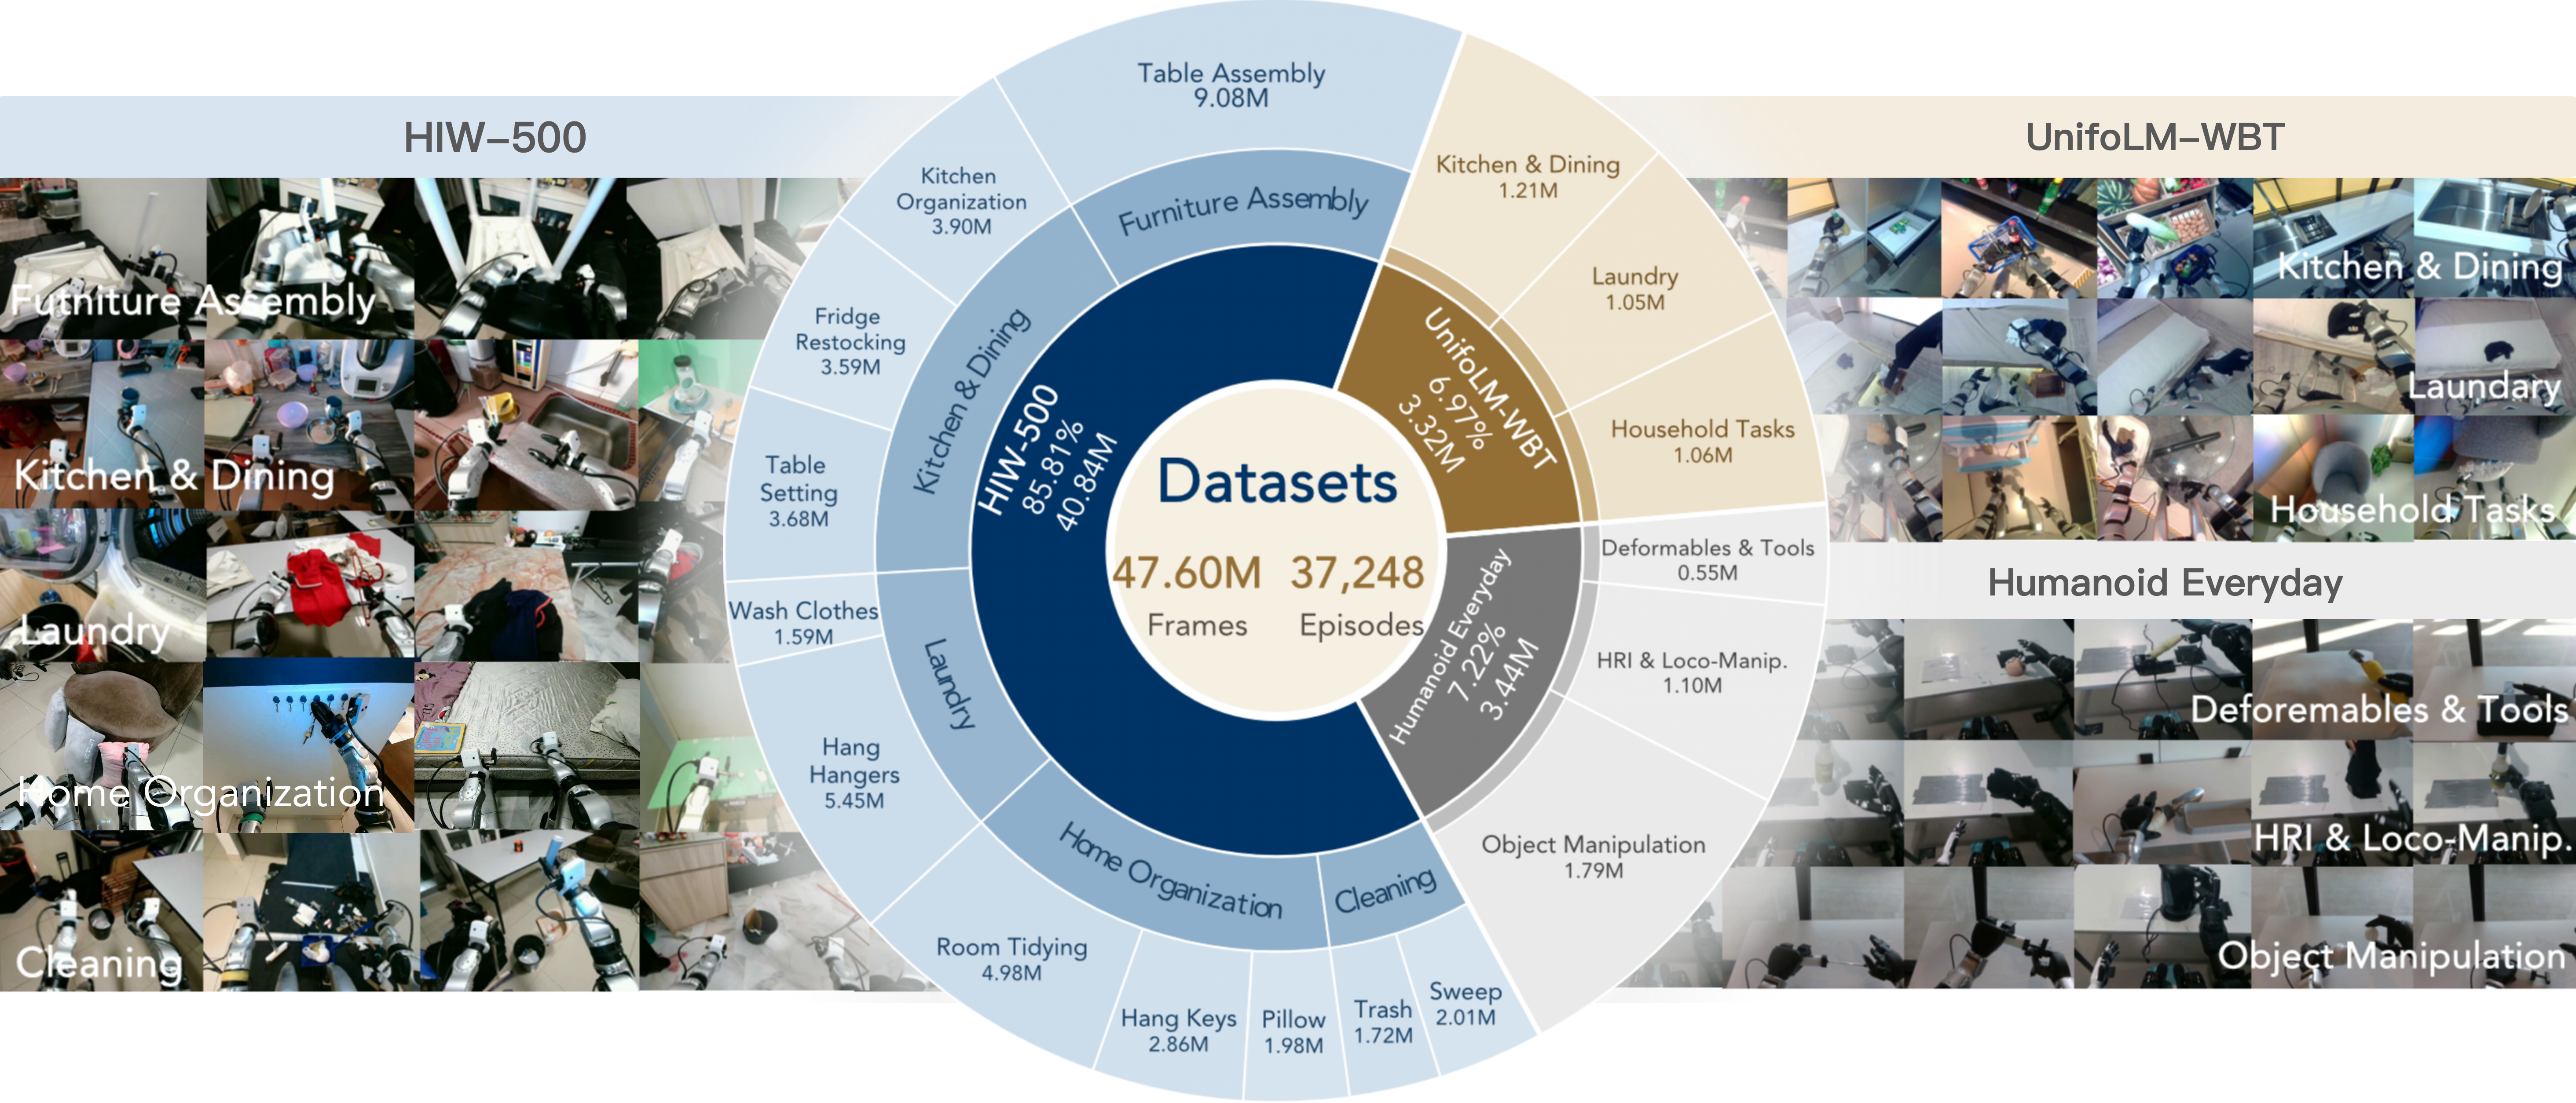
\includegraphics[width=\textwidth]{image/pretrain.png}
  \caption{\textbf{Composition of the VLA Pretraining Corpus.} The corpus combines HIW-500, 14 task subsets from UniFoLM-WBT available when the corpus was assembled, and Humanoid Everyday. UniFoLM-WBT entries released after corpus construction are excluded.}
  \label{fig:pretraining_datasets}
\end{figure}

\textbf{Implementation Details.} We pretrain the policy for 1,000k optimization steps on 16 NVIDIA H200 GPUs, taking approximately 60 hours with bfloat16 mixed precision and a global batch size of 1024. During VLA pretraining, hand supervision is represented as a two-dimensional binary vector indicating the open/closed state of the left and right hands. This shared representation accommodates the different hand morphologies, degrees of freedom, and control conventions in the source datasets, preserving grasp-and-release semantics while providing a consistent target for the hand head. We use AdamW with learning rates of $3\times10^{-5}$ for the ControlNet backbone and $1\times10^{-4}$ for the ControlNet adapters and hand head, together with a weight decay of $0.01$. The learning rate follows a cosine schedule with 1\% warm-up and a minimum of 10\% of its initial value.

\subsection{Post-Training}
\label{sec:setup_posttraining}
\textbf{HumanoidArena Benchmark.} HumanoidArena~\cite{humanoidarena,sonic} provides seven leg-critical tasks: three human--object and four human--scene interaction tasks requiring coordinated locomotion, balance, posture adjustment, and manipulation. Its SONIC data contain 100 successful demonstrations per task (700 total) with synchronized egocentric RGB, proprioceptive states, and whole-body targets. We use all seven tasks for single-task fine-tuning and joint multi-task training, the latter being more challenging because one policy must acquire all tasks simultaneously. We evaluate closed-loop performance with SONIC using success rate (SR) and average fall rate (AFR), capturing both task completion and stability during whole-body task execution.

\textbf{SIMPLE Benchmark.} SIMPLE~\cite{simple} integrates MuJoCo contact dynamics with Isaac Sim rendering for scalable evaluation of humanoid loco-manipulation. The paper describes a benchmark comprising 60 tasks; of these, 18 have been released in the public codebase to date. The paper reports baseline results for six tasks, with two evaluated using AMO and four using the SONIC tracker. From the currently released tasks, we select eight for evaluation: Handover, Mobile P\&P, XMoveBendPick, CloseDoor, OpenOven, OpenFaucet, Push Office Chair, and OpenTrashCan. Together, these tasks cover object handover, mobile pick-and-place, articulated-object interaction, and household-object manipulation, allowing us to assess policy robustness and execution stability in contact-rich whole-body control.

\textbf{Real-World Data Collection and Setup.} We collect real-world demonstrations with a teleoperation system implemented on top of and extended from the NVIDIA Isaac-GR00T data-preparation pipeline~\cite{grootn1}. As shown on the left of Fig.~\ref{fig:real_world_setup}, the operator uses a PICO 4 Ultra headset and hand controllers together with PICO body trackers for whole-body and lower-limb tracking. The humanoid is equipped with an Intel RealSense D435i camera and Dex3-1 dexterous hands. We define eight real-world tasks spanning locomotion, balance, and single- and dual-arm manipulation, and record 25--30 demonstrations per task. The two plots on the right of Fig.~\ref{fig:real_world_setup} show representative joint-position traces from two of these tasks: in Football Scoring (Fig.~\ref{fig:real_world_setup}a), the right-leg trajectory changes sharply around the kick, while in Banana Cabinet (Fig.~\ref{fig:real_world_setup}b), the traces vary across the pick, place, and push phases. In both plots, solid curves show measured joint positions and dashed curves show the corresponding action commands for the left and right sides, illustrating the task-dependent motion captured in the demonstrations. We store the demonstrations in a LeRobot v2.1~\cite{cadene2026lerobotopensourcelibraryendtoend}-compatible format, extended with Kimodo-specific motion and control fields for policy training with a motion prior.

\begin{figure}[H]
  \centering
  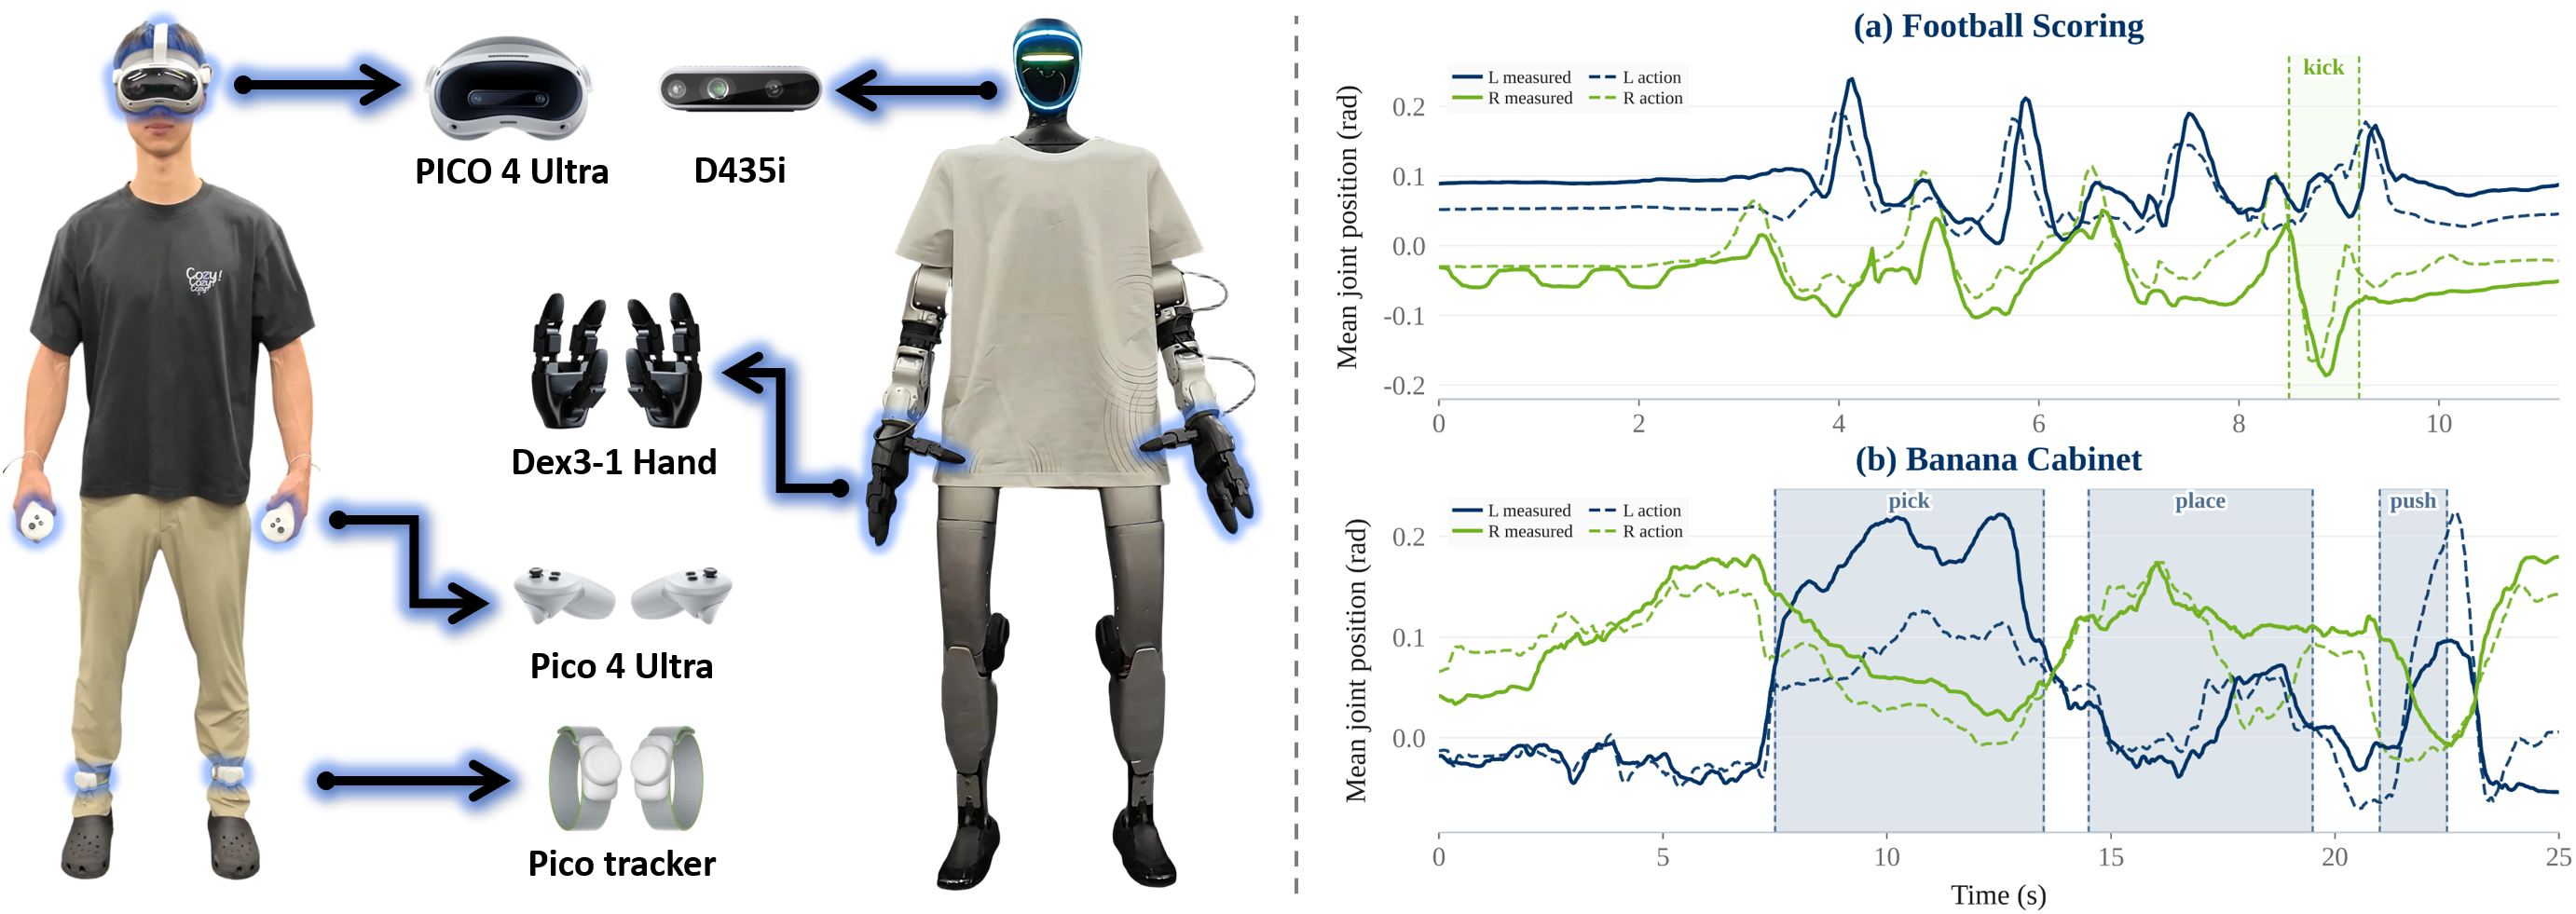
\includegraphics[width=\textwidth]{image/post-train.png}
  \caption{\textbf{Real-World Data Collection and Motion Profiles.} Left: PICO-based whole-body teleoperation of the humanoid. Right: measured (solid) and commanded (dashed) left- and right-side mean joint positions for two of the eight physical-robot tasks: (a) Football Scoring, showing a pronounced right-leg change during the kick, and (b) Banana Cabinet, showing motion across the pick, place, and push phases.}
  \label{fig:real_world_setup}
\end{figure}

\textbf{Implementation Details.} We fine-tune all policies with bfloat16 precision on four GPUs using 30\,Hz motion sequences, a 100-frame history, and a 50-frame prediction horizon. HumanoidArena single-task policies use a global batch size of 64 for 200k steps, while the joint seven-task policy uses a batch size of 128 for 500k steps; SIMPLE uses a batch size of 64 for 200k steps, and real-world policies use a batch size of 32 for 50k steps. Scratch-trained and VLA-pretrained variants share the same fine-tuning setup and differ only in initialization. The four-layer ControlNet detaches the root-control input to body prediction. We train with an MSE objective weighted 4, 1, 1, and 0.2 for root motion, body motion, hand control, and hand transitions, respectively, using AdamW (weight decay 0.01) and a cosine schedule with 1\% warm-up and a 10\% minimum learning-rate ratio. The ControlNet backbone, adapters, and hand head use learning rates of $3\times10^{-5}$, $1\times10^{-4}$, and $1\times10^{-4}$ for HumanoidArena and real-world fine-tuning, and $1\times10^{-5}$, $3\times10^{-5}$, and $3\times10^{-5}$ for SIMPLE. SIMPLE training uses color jitter and continuous hand-control targets; real-world training uses color jitter and random crops, with binary hand commands conditioned on measured hand closure. At inference, all policies run on one NVIDIA RTX 4090 with 10 diffusion denoising steps and predict a 50-frame action horizon at 30\,Hz. We execute 15 predicted frames per policy update on HumanoidArena and the real robot, and either 15 or 50 frames on SIMPLE depending on the evaluation setting. The SONIC tracker runs at 50\,Hz; real-time correction (RTC)~\cite{rtc} is enabled only for real-world deployment and disabled for HumanoidArena and SIMPLE.
